\documentclass[oxford]{ahsan}

\usepackage[backend=biber,style=numeric,citestyle=numeric]{biblatex} 
\addbibresource{references.bib} 

\title{\vspace{-3em}{Part C Project Report}\vspace{-1em}}

\begin{document}

\maketitle
\vspace{-3em}
\section{Project Overview}

Most modern real-time operating systems (RTOS) for small microcontrollers allow a
limited number of processes to run simultaneously, typically defined at compile time.
However, this restricts the flexibility to create processes dynamically. In contrast,
one of the earliest examples of an RTOS, deployed on the Apollo Guidance Computer
(AGC), allowed latency-insensitive jobs to be declared at runtime while processes with
stricter timing constraints were defined at compile time. The queue of processes
scheduled to run at predefined intervals was called the \texttt{WAITLIST}. Longer
\texttt{EXECUTIVE} jobs could be created dynamically with varying priorities, often
initiated by \texttt{WAITLIST} jobs, and were executed using the remaining available
processor time.

This flexible design made the AGC highly fault-tolerant. Famously, during the Apollo 11
landing, the AGC in the lunar module ran out of memory for new \texttt{EXECUTIVE} jobs,
triggering a \texttt{1202} alarm. While low-priority tasks, such as updating the
astronauts' displays, failed to execute, higher-priority jobs that controlled the
spacecraft continued unaffected, allowing the crew to land safely.

The goal of this project is to implement a real-time operating system that models this
approach on a small microcontroller and to explore the potential advantages of this
design over the commonly used round-robin schedulers in modern RTOS implementations.

\section{Progress}

The initial phase of the project involves implementing the AGC's scheduling algorithm
on a modern microcontroller. Based on the advice of my supervisor, Prof. Alex Rogers, I
selected the \texttt{micro:bit v1} device as the target platform. This device features
an ARM Cortex-M0 processor and includes peripherals such as system timers, LEDs, and a
radio module.

\vspace{-4em}
\begin{figure}[H]
    \centering
    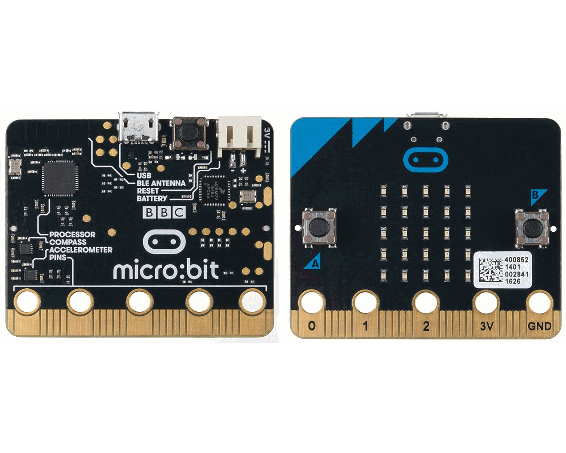
\includegraphics[width=.5\linewidth]{microbit.png}
    \vspace{-4em}
    \caption{A \texttt{micro:bit v1} device}
\end{figure}
\vspace{-1em}

To begin, I familiarized myself with programming microcontrollers at the bare-metal
level. I studied the book ``Bare-metal Programming for ARM'' \cite{baremetal-arm},
implementing its examples to gain hands-on experience. This process helped me quickly
get up to speed with microcontroller programming.

Next, I set up a development framework for working with the physical \texttt{micro:bit}
device. The book ``Bare Metal \texttt{micro:bit}'' by Mike Spivey \cite{microbit} was
particularly helpful, as it included hardware headers and reference manuals specific to
the \texttt{micro:bit}, enabling a quick and efficient setup. I also developed
automation tools to compile and deploy code to the \texttt{micro:bit} device directly
from my laptop.

After establishing the development environment, I began investigating the AGC scheduler
in detail. To deepen my understanding, I am studying the book ``The Apollo Guidance
Computer: Architecture and Operation'' by Frank O'Brien \cite{agc_book}. Currently, I
have a working implementation of the \texttt{WAITLIST} tasks, which employ a primitive
form of multiprocessing using timer interrupts. The next step is to implement
preemptive context switching and runtime process creation. Subsequently, I plan to
complete the implementation of \texttt{EXECUTIVE} jobs from the AGC. To efficiently
support priority-based multitasking with \texttt{EXECUTIVE} jobs, I intend to study
algorithms used by modern operating systems like Linux and implement a simplified
version tailored to the project.

To demonstrate the effectiveness of this scheduler, I plan to develop a minimal shell
for the operating system. This shell will enable basic scripting capabilities and
runtime process creation.

\section{Feedback}

Progress on my project has been slower than anticipated this term due to my commitments
to job hunting and PhD applications. However, I aim to accelerate during the Christmas
break. So far, I have had two meetings with Prof. Alex Rogers to discuss the project's
progress and direction. His feedback has been constructive and helpful, providing
valuable insights to guide my work.

\printbibliography

\end{document}
